%!TEX root = ../main.tex
%%%%%%%%%%%%%%%%%%%%%%%%%%%%%%%%%%
% Links:
%
% Difficulty:
% Companies: 
%%%%%%%%%%%%%%%%%%%%%%%%%%%%%%%%%%


%\begin{figure}
%   \centering
%   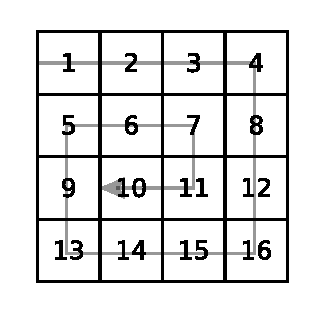
\includegraphics[width=\textwidth]{sources/spiral_matrix/images/example1}
%   \caption[Sample short cpation]{Sample Caption}.
%   \label{fig:spiral_matrix:example1}
%\end{figure}

\section{Spiral Matrix}
\label{ch:spiral_matrix}

\section{Problem statement}
Write a function that, given a matrix $M$ of size $m\times n$ returns a list containing the elements of $M$ in spiral order.
\begin{exercise}
\label{example:spiral_matrix:exercice1}

    %example1
    \begin{example}
        \label{example:spiral_matrix:example1}
        \hfill \\
        Given the matrix shown in Figure \ref{fig:spiral_matrix:example1}  the function returns \inline{1,2,3,4,5,6,7,8,9};
    \end{example}


    %example2
    \begin{example}
        \label{example:spiral_matrix:example2}
        \hfill \\
        Given the matrix shown in Figure \ref{fig:spiral_matrix:example2}  the function returns \\ \inline{1,2,3,4,8,12,16,15,14,13,9,5,6,7,11,10}.
    \end{example}

\end{exercise}
\begin{figure}[t]
    \centering
    \begin{subfigure}[]{0.45\textwidth}
        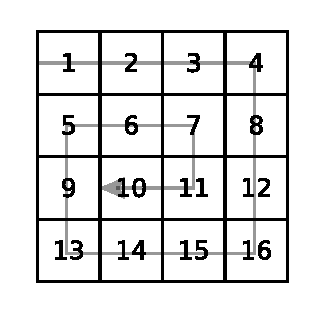
\includegraphics[width=\textwidth]{sources/spiral_matrix/images/example1}
        \caption[]{}
        \label{fig:spiral_matrix:example1}
     \end{subfigure}
    \hfill
    \begin{subfigure}[]{0.45\textwidth}
        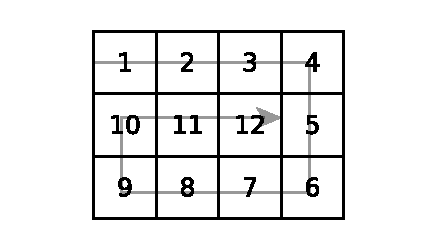
\includegraphics[width=\textwidth]{sources/spiral_matrix/images/example2}
        \caption[]{}
        \label{fig:spiral_matrix:example2}
    \end{subfigure}
\end{figure}



\section{Discussion}
\label{spiral_matrix:sec:discussion}
Let's start by noticing that our solution must return an array of size $m /times n$. 
This figure gives us a lower bound for the time and space complexities of any solution we can possibly come up with.

It is not difficult to solve this problem by hand with paper and pen and in fact if we have a go at solving one of the examples we might immediately realize that there is a clear pattern in the way the matrix is visited. 
In particular, we can see that we perform a number of rightward, downward, leftward, and upward sweeps on the matrix until we have no more rows and cols to visit. 
We can also notice that a movement is always either along a row or a column. 
For instance, w.r.t. Example \ref{ex:spiral_matrixexample1} we can see that the very first group of cells visited is the entire first row, followed by the cells in the last column, followed by the cells in the last row followed by the first column (minus the first cell which was visited already). 
When a sweep in a particular direction is completed the visited row or column should not be visited anymore in the future. 
When performing the first downward sweep in the example \ref{ex:spiral_matrixexample1} we see that no cells in the last column are ever visited again by any subsequent sweep.

We can build a solution solely on these observations. The solution will in practice visit one cell at a time and keep track of the type of sweep (left to right, top to bottom, right to left, or bottom to top) currently active to decide which cell to visit next. 

In order to avoid visiting already visited cells, we can use 2 pairs of integers: 
\begin{itemize}
    \item \inline{vertical_up_limit}:
    \item \inline{vertical_down_limit}:
    \item \inline{hotizontal_left_limit}:
    \item \inline{hotizontal_right_limit}:
\end{itemize}


\subsection{Brute-force}
\label{spiral_matrix:sec:bruteforce}

    \lstinputlisting[language=c++, caption={Sample Caption},label=list:spiral_matrix]{sources/spiral_matrix/spiral_matrix_solution1.cpp}

